%
% latex-sample.tex
%
% This LaTeX source file provides a template for a typical research paper.
%

%
% Use the standard article template.
%
\documentclass{article}

% The geometry package allows for easy page formatting.
\usepackage{geometry}
\geometry{letterpaper}

% Load up special logo commands.
\usepackage{doc}

% make a reference to Hypertext 
\usepackage{hyperref}

% Package for formatting URLs.
\usepackage{url}

% Packages and definitions for graphics files.
\usepackage{graphicx}
\usepackage{epstopdf}
\DeclareGraphicsRule{.tif}{png}{.png}{`convert #1 'dirname #1'/'basename #1 .tif'.png}

%
% Set the title, author, and date.
%
\title{{Trends in Worldwide Refugee Migration}  
\\ 
\small{DNSC 6211: Programming for Analytics}}
\author{Jessica Smith}
\date{12/7/2015}

%
% The document proper.
%
\begin{document}

% Add the title section.
\maketitle

% Add an abstract.
\abstract{
\noindent
Each year the World Bank (via the UN Refugee Agency) takes a data snapshot of the refugee population worldwide. Given the recent dislocation of millions of people due to war and regional instability, I chose to explore this data in depth. My objective was to expand my understanding of the historic trends leading up to the current refugee crisis, and develop a tool that would allow others to do the same. I used Python to extract and explore data, and then created an R Shiny application to showcase trends in year-by-year interactive visualizations as well as static tables. The data reveal startling jumps in the number of worldwide refugees in recent years, and a simultaneous decrease in the population of refugees in the United States. Alarming trends, particularly in Syria and Afghanistan, point to a burgeoning crisis and massive waves of migration that are unlikely to dissipate in the immediate future. \vspace{2mm}

\noindent A video walk-through of this project is available at \url{https://youtu.be/m9PmDfIXqk0}\vspace{2mm}

\noindent This project is also available on GitHub at \url{https://github.com/JASmith0820/Refugee_Data_R_Shiny_App}
}

% Add various lists on new pages.
\pagebreak
\tableofcontents


% Start the paper on a new page.
\pagebreak

%
% Body text.
%
\section{Introduction}
\label{introduction}

With both longstanding regional conflict and the ongoing Syrian civil war continuing to displace millions of people, the matter of where to shelter refugees presents a critical, yet unanswered question. Some countries are responding by shutting borders, while others are opening their doors. The world must decide how to respond to the growing number of refugees, and a deeper knowledge of the history of refugee movements and the scale of the current crisis may add meaningful insight to the conversation. For this reason I chose to focus my project on the historical refugee data gathered by the World Bank.\vspace{2mm}

\noindent The overarching question driving my research was "What is the scale of the refugee crisis today as compared with other moments in history? Have we seen mass migration on this scale in recent decades, or is today's situation relatively unprecedented?" To answer this question, I built an R Shiny application that allows users to browse through charts and graphs detailing refugee data over the past twenty years. Users can delve into historic data to broaden and deepen their contextual understanding of today’s refugee numbers.  

\section{Background}

The World Bank collects data annually on the number of reported refugees by country of origin and by country of asylum. I had hoped to review a longer time period, perhaps the past 100 years, but unfortunately the World Bank's data is quite sparse prior to the mid-1990s. As a result I limited my scope to the past 20 years. As my driving goal was understanding how today's refugee population compares with that of previous years, I began with simple charts showcasing the worldwide number of refugees broken out by country of origin in each year.\vspace{2mm}

\noindent
Another question soon presented itself: Instead of focusing on solely the raw numbers, could I determine which countries had the highest \emph{proportion} of refugees leaving? Could there be a smaller country experiencing a large exodus that would not appear in the first graphs simply because of the original population size? To calculate refugees as a proportion of total population I downloaded a World Bank indicator detailing Total Population per country per year.\vspace{2mm}

\noindent
After spending some time reviewing these data, a new question arose: How has the refugee population in the United States changed in the past 20 years? As the number of worldwide refugees grows does the U.S. have a higher or lower number of refugees?
These were the primary questions driving my research, and I determined that an R Shiny app would be the best tool for presenting these data.
\section{Method}

First I wished to assess the level of dislocation in terms of sheer volume. I created one plot showing the top 10 countries from which refugees had left, and a second showing the top 10 countries in which refugees had received asylum. This provided both an overall sense of the total scale of dislocation and indicated which countries were the most active participants (either as countries of origin or asylum).
Next, I created two tables focused on proportionality rather than raw numbers by dividing the number of refugees by the total given population in that year. Again, I limited the tables to the top 10 highest countries. These and the plots mentioned above provide one year of data at a time. \vspace{2mm}

\noindent
I also wished to create some static charts to pinpoint critical trends without requiring users to scroll through the data year by year. I examined the top ten countries and years with the highest refugee populations (one chart for country of origin, another for country of asylum). Finally, I created a static graph detailing the refugee population each year in the United States specifically.

\subsection{Workflow}

\begin{figure}[hb]
  \centering
    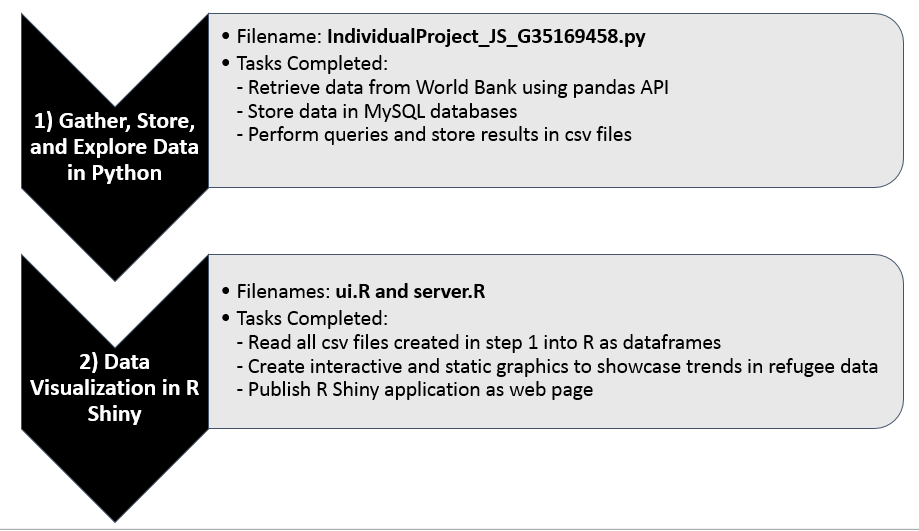
\includegraphics[scale=0.5]{Indiv_Project_Workflow}

\end{figure}


\noindent First, I used Python and the World Bank pandas API to retrieve the three indicators (refugee population by country of origin, refugee population by country of asylum, and total population). After performing some transformations to the data (merging all indicators into a single dataframe, removing null values) the data were loaded into a MySQL database. Continuing to work in Python, I ran several queries on the MySQL database and stored the results in csv files. \vspace{2mm}

\noindent
Next, I created an R Shiny application that read each of the files created above and displayed their data as either a plot or a table.
To recreate my steps, please ensure that the following are accessible by your working directory:

\begin{itemize}
\item Individual\textunderscore Project\textunderscore JSG35169458.py

\item ui.R

\item server.R
\end{itemize}

\noindent To begin, run the Individual\textunderscore Project\textunderscore JSG35169458.py code. Upon completion you should see 10 new csv files appear in your working directory. Please ensure that these are available in your working directory for the R Shiny app to read.
Next, re-create the R Shiny app by completing the following:

\begin{itemize}
\item In R, set your working directory to the directory in which the csv files and ui.R/server.R files are stored.

\item Load the shiny library ["library(shiny)"].

\item Run the application ["runApp()"].
\end{itemize}

\noindent Alternately, you can access the R Shiny app from the webpage to which it has been published at: \url{https://jasmith0820.shinyapps.io/Refugee_Shiny_App}\vspace{2mm}

\noindent A video walk-through of the project and R Shiny application is available at \url{https://youtu.be/m9PmDfIXqk0}

\subsection{Project structure}

\noindent Three World Bank Indicators were used to complete this project:

\begin{itemize}
\item \textbf{Refugee population by country or territory of asylum:}\\
\url{http://data.worldbank.org/indicator/SM.POP.REFG} \\
\noindent The World Bank defines this population as individuals recognized as refugees based on international standards, as well as those granted refugee-like humanitarian status and those provided temporary protection. Individuals who have applied for asylum but have not yet received a decision are excluded. Country of asylum is the country in which the asylum claim was filed and granted.
\item \textbf{Refugee population by country or territory of origin:}\\
\url{http://data.worldbank.org/indicator/SM.POP.REFG.OR}\\
\noindent The same definition of refugee applies in this indicator as well. However, country of origin refers to the country of citizenship of the individual who is claiming asylum.
\item \textbf{Population, total:}\\
\url{http://data.worldbank.org/indicator/SP.POP.TOTL}\\
\noindent The World Bank defines this as the count of all residents regardless of legal status or citizenship. Refugees who are not yet permanently settled in the country of asylum are excluded. The value represents a midyear estimate.
\end{itemize}
\noindent The total population indicator is used solely for calculating proportions. The other two indicators are the data sources used to answer all other research questions. The indicators were downloaded for all countries in the years 1995 to 2014. Countries which failed to provide data are excluded, and a list of excluded countries in each year appears in the R Shiny application.


\subsection{Figures and Tables}

\noindent There are several figures in the R Shiny application. The first figures are interactive and present annual data as users scroll through different years. The remainder are static and show aggregate trends over the entire timeframe.\vspace{2mm}


\noindent Interactive figures:
\begin{itemize}
\item \textbf{Total refugees counted worldwide}: The aggregate sum of the number of refugees worldwide (calculated using the country of asylum data)
\item \textbf{Total refugee population in the USA}: The total number of refugees currently living in the United States
\item \textbf{Where did refugees leave?}: Bar chart breaking down the worldwide refugee population by country of origin (top ten highest displayed)
\item \textbf{Where are refugees now?}: Bar chart breaking down the worldwide refugee population by country of asylum (top ten highest displayed)
\item \textbf{Missing countries}: Each year certain countries fail to provide data, and therefore are excluded; this table indicates which were excluded in the given year
\item \textbf{Highest proportion leaving}: Calculates the number of refugees who left the country as a proportion of the total population in that year; displays the top ten highest
\item \textbf{Highest proportion arriving}: Same as above, but for countries of asylum
\end{itemize}
\noindent Static figures:
\begin{itemize}
\item \textbf{All-time highest number leaving}: A ranking of the countries and years with the highest refugee population by country of origin
\item \textbf{All-time highest number arriving}: Same as above, but for countries of asylum
\item \textbf{Number of refugees granted asylum in the USA}: The refugee population in the United States each year
\end{itemize}

\section{Discussion}

\noindent The R Shiny application reveals several interesting points about the evolution of the Syrian refugee crisis. Leading up to 2012 Syria was one of the top destinations for refugees, annually sheltering a population of around 1.5 million asylum-seekers from other nations. The tide turned in 2012, when refugees began pouring out of Syria. In 2012 there were 729,000 Syrians seeking asylum elsewhere, the 4th-highest number in the world. The population of Syrians seeking asylum outside of Syria surged to 2.4 million in 2013, and then to 3.8 million in 2014, setting a record for the highest number of refugees from a single country since 1995.\vspace{2mm}

\noindent A similar jump occurred in Afghanistan between 2000 and 2001. The late 1990s saw relatively low levels of refugees worldwide. But in 2001, the number of Afghans seeking asylum outside of Afghanistan jumped to 3.8 million, nearly matching the record high held today by Syria. The number dropped the following year to about 2.5 million, but Afghanistan remained above 2 million through 2014.\vspace{2mm}

\noindent 
Since 1995 the refugee population in the United States has been declining. In 1995 the United States was home to 623,294 refugees, while in 2014 the population had dimished to 267,222. 2014 represented a moderate increase from the lowest population point of 262,023 in 2012, but is still very low compared to historic rates and the worldwide number of refugees.


\subsection{Learnings}

\noindent In order to understand the World Bank's data I had to spend a lot of time familiarizing myself with the definition of a refugee, and the policies surrounding the numbers. For example, the U.S. refugee population displays a sudden jump from 379,340 in 2005 to to 843,498 in 2006. I could not find any data indicating that the number of accepted refugees increased, and was at a loss to explain this jump. However, exhaustive research in the UNHCR's website revealed that in 2006 the agency changed it's definition of refugee to include individuals in resettlement programs. The next year it changed the definition back to its original form, which excluded those programs. (This explanation was found on page 11 of the UNHCR 2007 yearbook: \url{http://www.unhcr.org/4981c4812.html}) Without background knowledge of refugee policies these types of trends are extremely confusing. Despite the challenge it posed, it was gratifying to learn so much about refugee policies, and I would like to continue exploring this in the future. \vspace{2mm}

\noindent Regarding programming skills, this project taught me a great deal about working with APIs, storing and retrieving data from MySQL databases in Python, using ggplot, and the inner workings of R Shiny applications. 

\subsection{Challenges}

\noindent The biggest challenge with the data was that it was a population snapshot rather than a description of the inflow and outflow of refugee populations. For example, I can see that Jordan is home to approximately 2 million refugees a year. However, I cannot determine whether this is a static population or a large volume of refugee traffic passing in and out of the country. The insights revealed could have been richer if inflow/outflow data were available. In addition, I could not see which refugees ultimately ended in which country of asylum. It would have made for a more interesting analysis if I could trace refugees to their ultimate destination, instead of simply looking at overall patterns. 

\section{Conclusion}

\noindent My primary goal was to create a tool exploring the historical context and scale of today's refugee crisis. I explored data about where refugees left and where they went during the twenty years between 1995 and 2014, including trends in the United States specifically. I learned that a record number of Syrians sought asylum in 2014, while the refugee population in the United States was at a historic low. A similar exodus occurred in Afghanistan in 2001, and more than a decade later Afghanistan continues have a large population of individuals seeking asylum elsewhere. In light of these data, I concluded that today's refugee crisis reflects a uniquely devastating level of displacement, and if these trends continue, will remain an extraordinary challenge for decades to come. The refugee crisis is far from over, and a solution must be found to avoid further destabilization to an already fraught region.


\end{document}

